\subsection{Authentication}

\subsubsection{scope}
\par{This module takes care of everything involving the users account. This includes functionality like logging in and out of the system, editing of user accounts etc. Further description is provided in the use cases below}

\begin{figure}[h]
	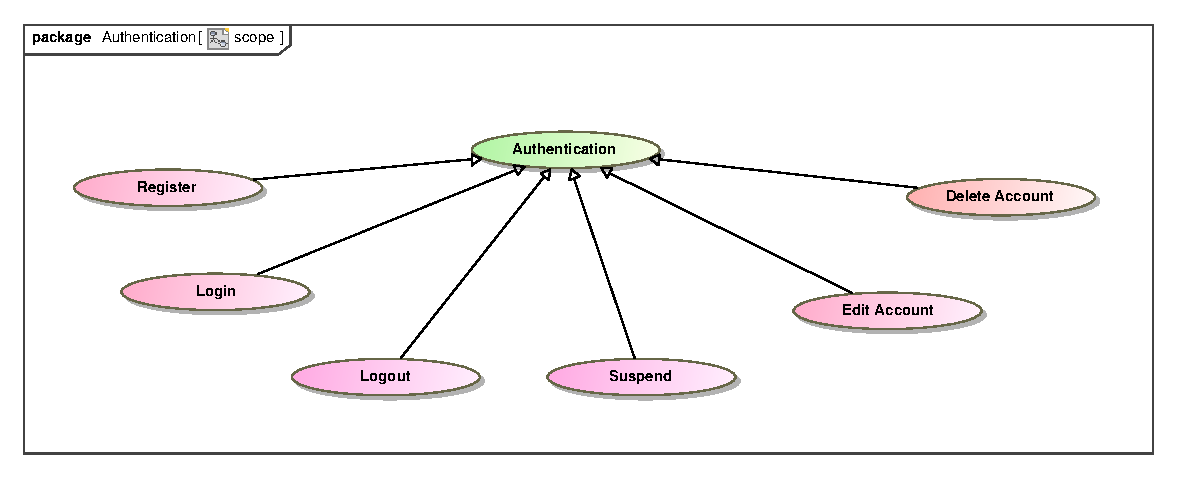
\includegraphics[scale=0.9]{epsImages/Authentication/AuthenticationScope.eps}
	\caption{Scope for authentication module}
\end{figure}

\newpage
\subsubsection{Use Cases}

\begin{enumerate}

\item \textbf{registerAccount  – priority: critical } 
This use case creates  a user account that gets persisted to database.

\textbf{Service Contract:}

\begin{figure}[h]
		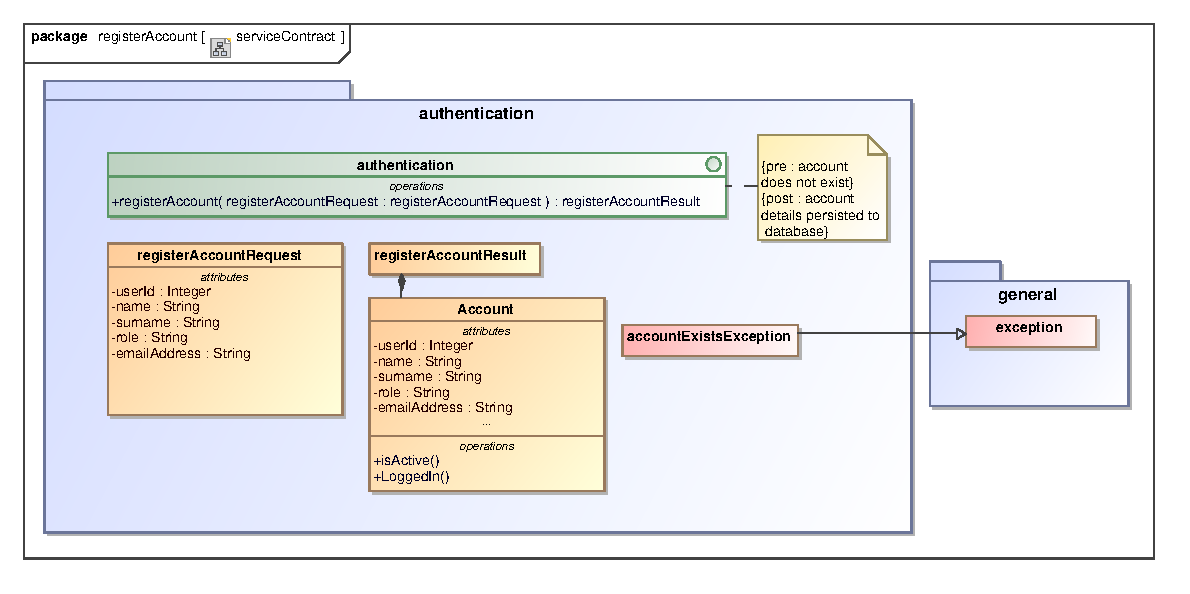
\includegraphics[scale=0.9]{epsImages/Authentication/serviceContract.eps}
		\caption{Service contract for registering new user account}
\end{figure}

\newpage
\item \textbf{Login - priority: critical}
This use case allows a user to log into an existing account.

\par{\textbf{Service Contract} The service contract for the login service is shown in figure below.}
\begin{figure}[h]
		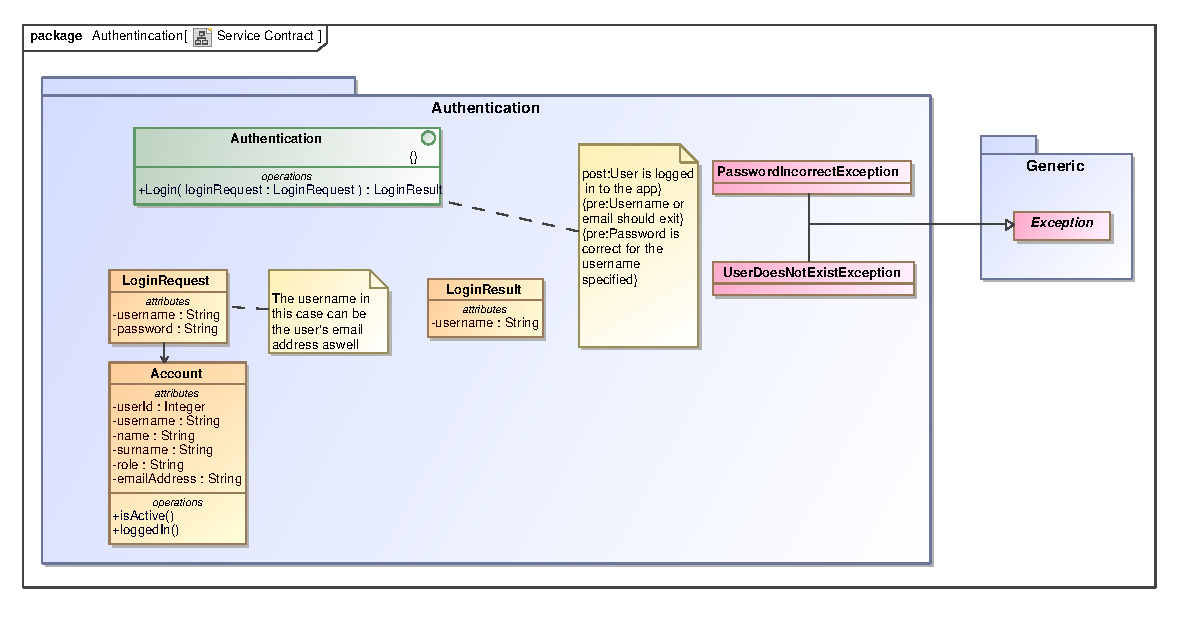
\includegraphics[scale=0.9]{epsImages/Authentication/LoginServiceContract.eps}
		\caption{Service contract for logging into a user account}
\end{figure}

\item \textbf{Logout - priority: important} \\
This use case allows a user to log out of the system safely. \\ \\

\textbf{Service Contract:}
\begin{figure}[h]

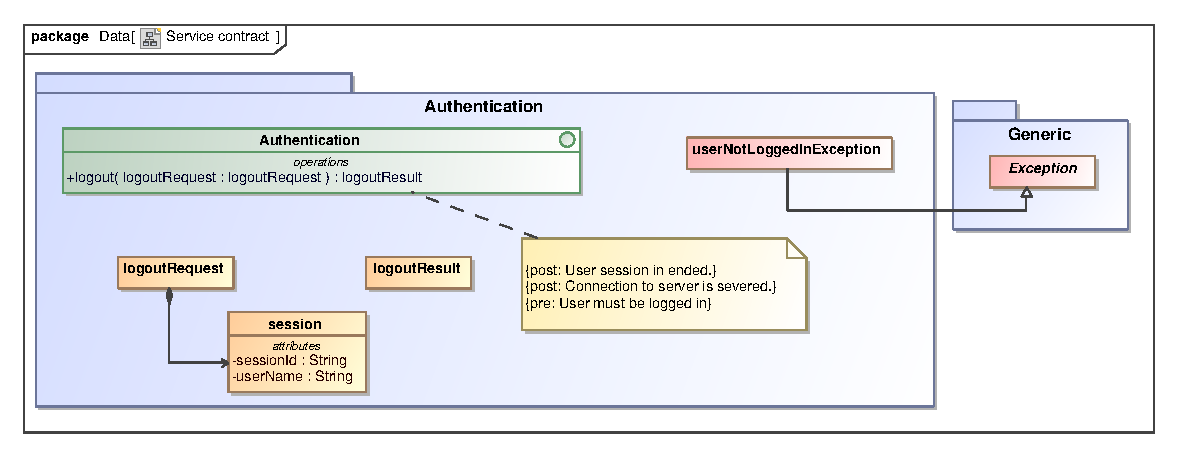
\includegraphics[scale=.9]{epsImages/Authentication/logoutServiceContract.eps}
\caption{Service contract for logging a user out of the system}
\end{figure}

\newpage
\item \textbf{editAccount - priority: important}
	\par{This allows a user to make changes to their profile details. They will be allowed to edit the details they added when creating the account.}\\ \\
	
	\textbf{Service Contract:}\\
	\begin{figure}[h]
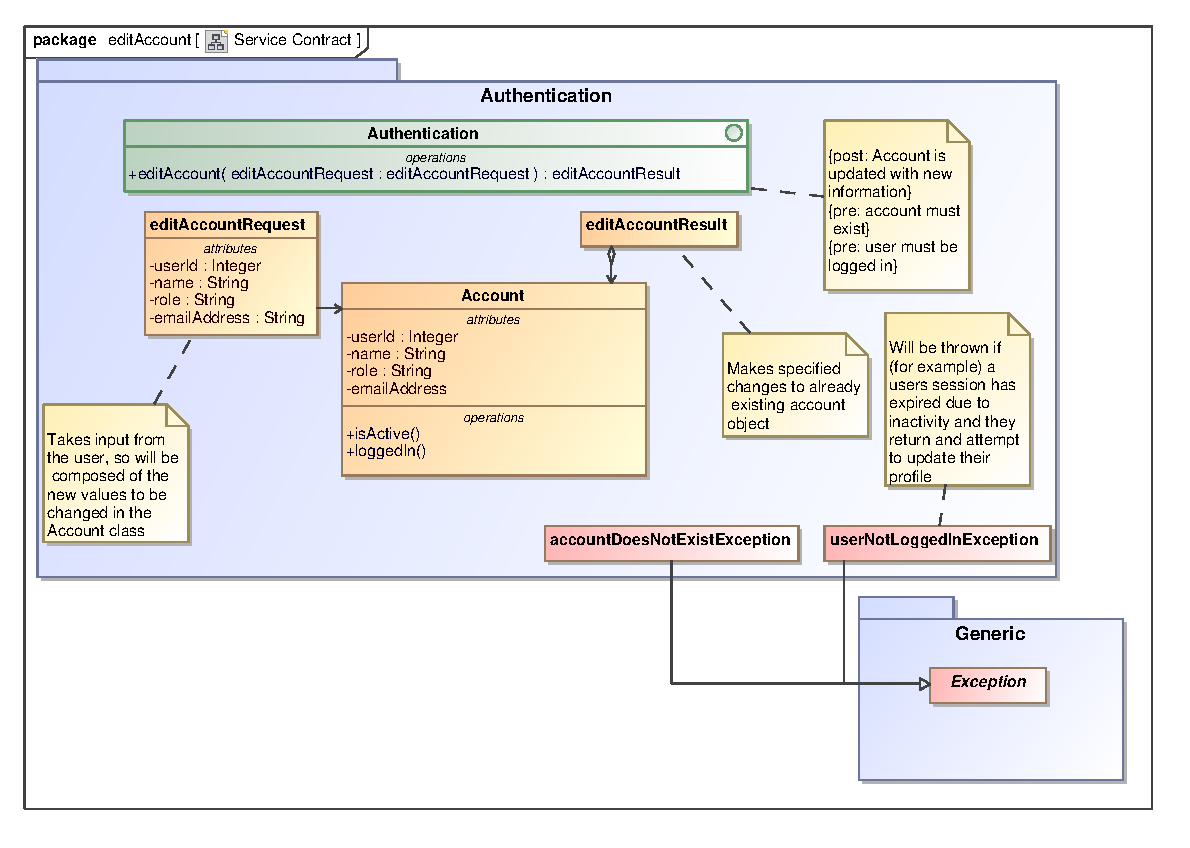
\includegraphics[scale=0.9]{epsImages/Authentication/editAccountServiceContract.eps}
\caption{Service contract for editing a users account}
\end{figure}

\newpage
\item \textbf{deleteAccount  – priority: important} 
This use case creates  a user account that gets persisted to database.

\textbf{Service Contract:}

\begin{figure}[h]
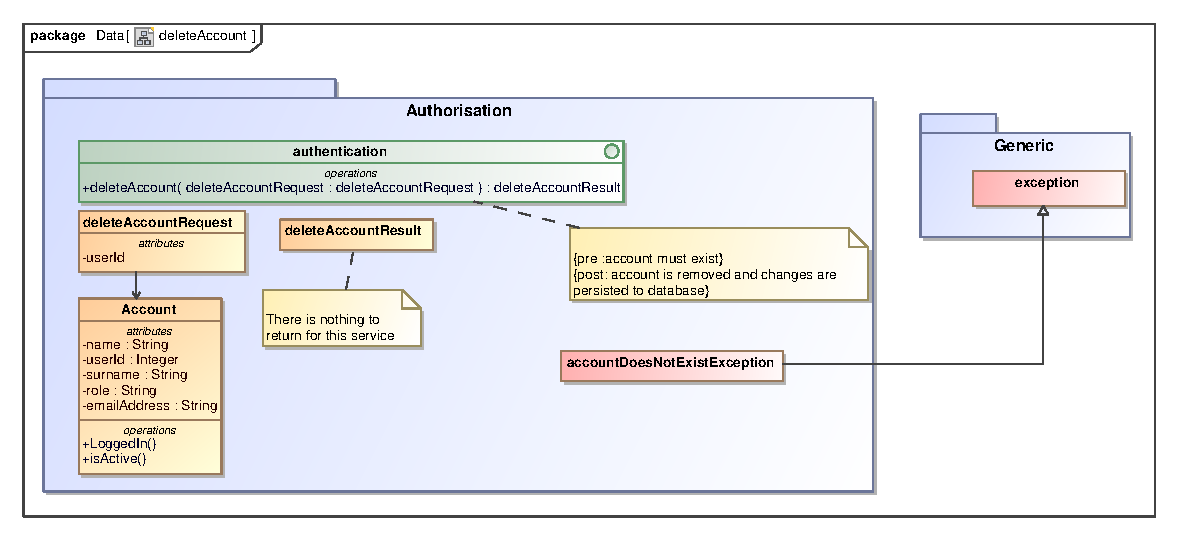
\includegraphics[scale=0.9]{epsImages/Authentication/deleteAccount.eps}
\caption{Service contract for deleting a users account}
\end{figure}

\newpage
\item \textbf{SuspendAccount - priority: important}\\
\par{This use case allows the system administrator to suspend a users account for any reason he/she may see as appropriate. A suspended account bars the user from logging in and/or using the account until the administrator lifts the suspension.}\\ \\

\textbf{Service Contract:}

\begin{figure}[h]
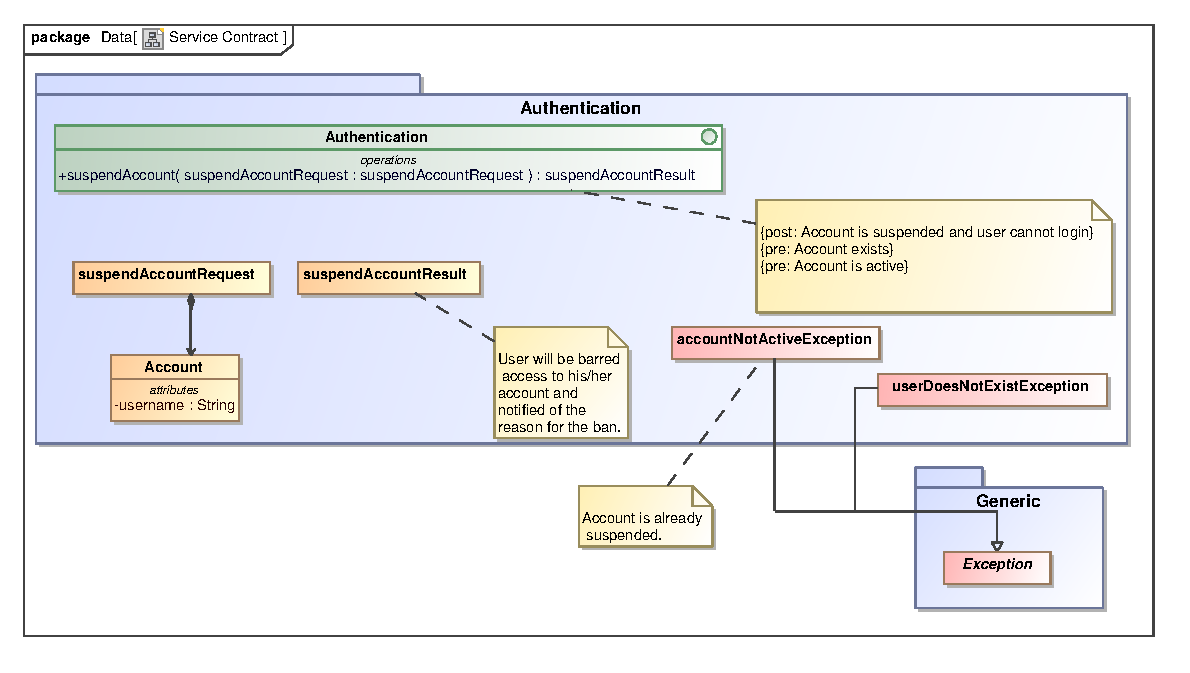
\includegraphics[scale=0.9]{epsImages/Authentication/suspendServiceContract.eps}
\caption{Service contract for suspending a users account}
\end{figure} 
\end{enumerate}

\newpage
\subsubsection{Domain Model}
\par{ The Authentication module will keep Account objects in the database. Any part of the system that checks for user authorisation will check against the account table to see if that particular user has authorisation to do whatever it is they are attempting to do. }

\begin{figure}[h]
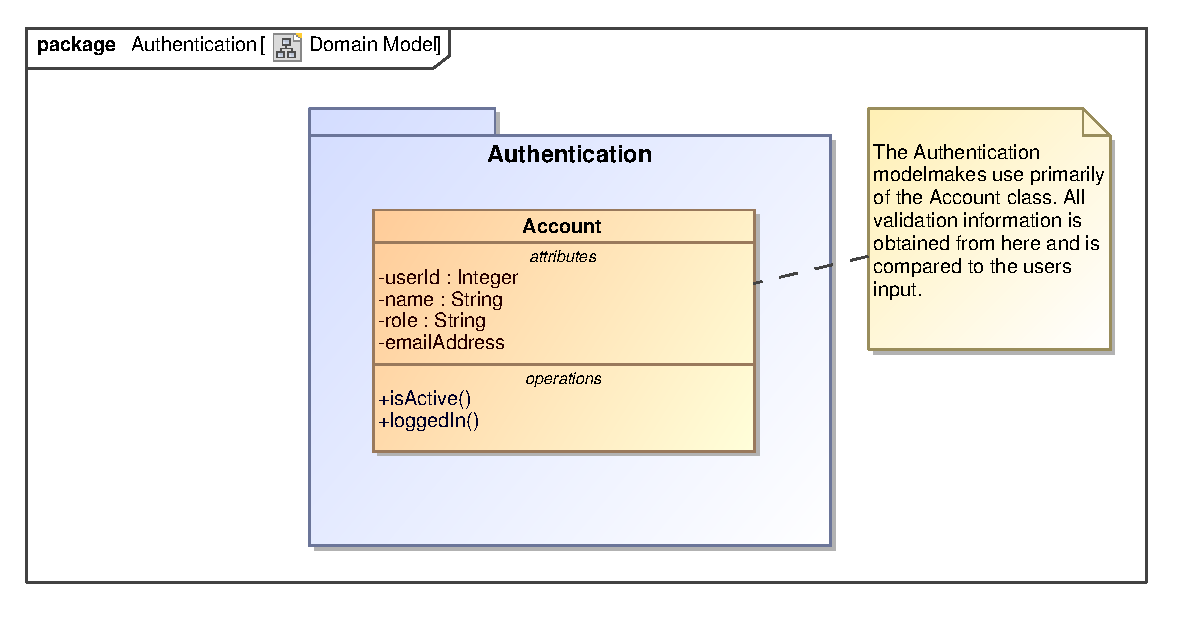
\includegraphics[scale=0.9]{epsImages/Authentication/domainModel.eps}
\caption{Domain model of Authentication module}
\end{figure}
